\section{Introduction}
\label{sec:introduction}

\begin{figure}[t]
\centering
%\includegraphics[width=0.94\textwidth]
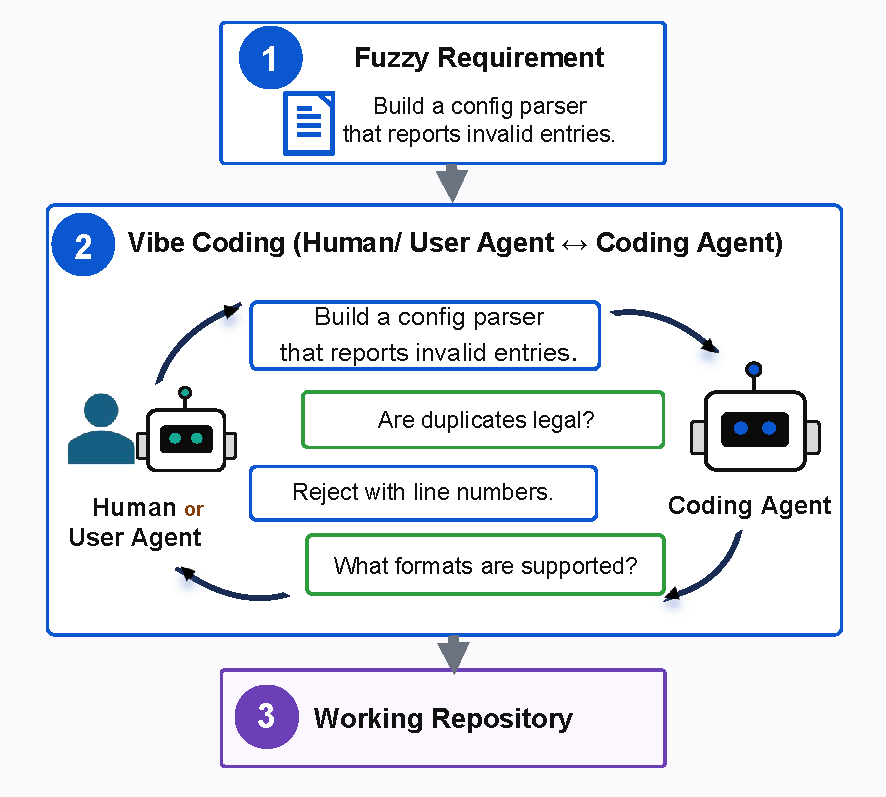
\includegraphics[width=0.94\columnwidth]{figures/vibe_coding_overview.pdf}
\caption{\textbf{Overview of the interactive requirement clarification setting of \rcb{}.} Given an ambiguous requirement, vibe coding resolves missing design decisions through dialogue between a human and a coding agent. 
Our benchmark simulates this process with a user agent that answers clarification questions and guides the coding agent toward a complete, testable specification, which is then used to build a working repository.}
\label{fig:user-agent-interaction}
\end{figure}

Coding agents are shifting from code assistants to project builders. Early research largely centered on local tasks, such as completing a function or suggesting an edit.
By contrast, as shown in Figure~\ref{fig:user-agent-interaction}, recent ``vibe coding'' workflows often begin with a high-level user intent, instead of a complete and clear implementation contract. The coding agent must clarify missing requirements, inspect files, run commands, edit repositories, install dependencies, iterate over execution failures, and ultimately deliver a working project~\cite{yang2024sweagent,openhands}. This makes it increasingly plausible for users to delegate not only coding steps, but also larger parts of the software construction process. 
In this setting, the central question is whether a coding agent can turn incomplete human intent into functioning software.

%The central question of this paper is simple: \emph{can coding agents ask the right questions before they write the wrong code?} Large language models are rapidly changing how software is written. Modern coding agents can inspect files, run commands, edit repositories, and iterate over failures, making it increasingly plausible for users to describe a desired product and delegate the implementation process to an agent~\cite{yang2024sweagent,openhands}. This practice is often closer to exploratory product development than to traditional code completion: the user may provide only a high-level intent, the exact interface may be negotiable, and many constraints become explicit only after follow-up questions.
%Large language models are rapidly changing how software is written. As coding agents become more capable, able to inspect files, run commands, edit repositories, and iterate over failures, a new style of development often called "vibe coding" is becoming increasingly common: a user describes a desired product in a few informal sentences and delegates the entire implementation to an agent. A pressing question arises: can current benchmarks actually tell us whether an agent fully captures what the user wants and successfully builds a project from scratch?

%This shift also changes what coding benchmarks should evaluate. Function-level benchmarks and repository-editing benchmarks measure localized synthesis, context use, and tool use inside existing codebases. From-scratch generation benchmarks move closer to project construction, but many still provide detailed requirements, fixed scaffolds, language-specific constraints, or explicit test contracts~\cite{zhao2024commit0,ding2026nl2repobench,fu2025prdbench}. These choices make evaluation tractable, but they remove the main difficulty of vibe coding: success requires a capability chain that begins with recognizing ambiguity, asking targeted questions, recovering hidden constraints, retaining them across development, and only then translating them into correct code. A benchmark for project-building agents should therefore evaluate more than static specification following.

This shift changes what coding benchmarks should evaluate, while existing ones still largely assume that the task goal is static, explicit, or discoverable without user interaction. Function-level benchmarks and repository-editing benchmarks measure localized synthesis, context use, and tool use inside existing codebases. From-scratch generation benchmarks move closer to project construction, but many still provide detailed requirements, fixed scaffolds, or language-specific constraints~\cite{zhao2024commit0,ding2026nl2repobench,fu2025prdbench}. 
A closely related step toward holistic software generation is ProgramBench~\cite{yang2026programbench}, which asks agents to rebuild programs from an executable and documentation. However, the target behavior is still exposed through a static interface. As a result, existing benchmarks remain limited in evaluating the broader capabilities required by vibe coding, where coding, planning, clarification, and iterative project construction are tightly coupled.

%Consider a user who asks for a small developer tool that ``parses configuration files and reports invalid entries.'' A detailed benchmark might immediately specify the file format, error schema, command-line interface, and all edge cases. A real user often does not. The agent must decide what is underspecified, ask whether duplicate keys are legal, clarify how syntax errors should be reported, and only then implement a robust tool. This example captures the setting targeted by \rcb{}: from-scratch repository generation under ambiguous product requirements.
%Consider a user who requests a small developer tool that "parses configuration files and reports invalid entries." A conventional benchmark would typically hand the agent a complete specification, including the file format, the error schema, the command-line interface, and every edge case to be handled. Real-world settings, however, rarely work this way: requirements tend to unfold gradually, evolving from vague to progressively clear. The agent must therefore determine for itself what remains underspecified—asking whether duplicate keys are legal, clarifying how syntax errors should be reported—and only then proceed to implementation.

%Existing coding benchmarks only partially capture this setting. Issue-resolution benchmarks such as SWE-bench evaluate agents inside an existing repository with a concrete bug report~\cite{jimenez2024swebench}. From-scratch generation benchmarks move closer to project construction, but they often provide detailed product requirement documents, implementation signatures, Python-only environments, or explicit test contracts~\cite{zhao2024commit0,ding2026nl2repobench,fu2025prdbench}. These design choices make evaluation tractable, yet they also create a semantic gap between benchmarks and real interactive development. In practice, a user rarely writes a complete architectural specification before implementation begins; instead, a capable agent should identify ambiguity, ask targeted questions, and revise its plan as the requirement becomes clearer.
%Existing coding benchmarks capture this setting only partially. On the one hand, some of them are file-level modification benchmarks operating within an existing repository. Issue-resolution benchmarks such as SWE-bench~\cite{jimenez2024swebench}, for instance, evaluate agents against a concrete bug report inside a codebase that is already in place. Such benchmarks cannot assess whether an agent can build a complete project from scratch, because the architecture, interfaces, and surrounding code are all given in advance. On the other hand, some benchmarks do support from-scratch project construction, but they depart from realistic conditions by handing the agent an unambiguous specification: detailed product requirement documents, implementation signatures, Python-only environments, or explicit test contracts~\cite{zhao2024commit0,ding2026nl2repobench,fu2025prdbench}. These benchmarks can only measure how well an agent implements a project once the requirements are already complete and clear. As a result, neither setting truly evaluates what matters in real-world development: whether an agent, starting from scratch and from an underspecified request, can pin down the user's actual intent and deliver a product that fully matches it. In practice, a user rarely writes a complete architectural specification before implementation begins. A capable agent should instead identify ambiguity, ask targeted questions, and revise its plan as the requirement becomes clearer.

%This gap creates a tension for benchmark design. If a benchmark provides detailed interfaces, implementation hints, and complete tests, then scoring becomes straightforward but the task is no longer realistic. If a benchmark provides only a concise requirement, then the task resembles real interactive development but evaluation becomes difficult because correct implementations may vary in language, architecture, and interface design. \rcb{} addresses this tension by separating \emph{requirement exposure} from \emph{behavioral evaluation}. The agent receives only a fuzzy product requirement document (PRD), a repository-specific ultimate image, and a small number of public examples. Evaluation, however, is performed through standardized black-box tests reconstructed from the original repositories, so a solution can be assessed without enforcing the original internal structure or programming language.

%We therefore introduce \rcb{}, an interactive benchmark for evaluating coding agents as project builders under ambiguous requirements.

In this paper, we introduce \rcb{}, an \textbf{I}nteractive \textbf{C}oding \textbf{A}gents \textbf{E}valuation \textbf{Bench}mark for vibe-coding workflows.
In each task, a tested coding agent starts from a fuzzy requirement and may ask an automated User Agent for clarification. The User Agent answers from hidden requirement records instead of free-form speculation. Under this design, the central difficulty is not merely that the initial requirement is vague, but that vagueness poses three key challenges.

%The first challenge is ambiguity vs. verifiability. A realistic project-generation task should begin from a fuzzy product intent, because real users rarely provide complete interface definitions, edge cases, or architectural constraints upfront. However, if a benchmark simply hand-writes vague requirements, failures become hard to interpret: the task may be underspecified, infeasible, or inconsistent rather than genuinely difficult for the agent. \rcb{} therefore does not create ambiguity by weakening task semantics. Instead, we begin with real open-source repositories whose original behavior is executable and testable, derive detailed product requirement documents and black-box behavioral tests from those repositories, and only then fuzzify the requirements by withholding selected constraints. The agent sees an ambiguous fuzzy product requirement document (PRD), but the benchmark retains a precise, executable specification for evaluation.
The first challenge is to ground ambiguity. In vibe-coding workflows, users rarely specify complete interfaces, edge cases, or architectural constraints upfront. However, if a benchmark directly writes vague requirements from scratch, the intended task may become underdefined. A failure may reflect an ambiguous or infeasible prompt rather than a limitation of the coding agent. We address this by deriving ambiguity from precision. Each task begins with a real open-source repository whose behavior is executable and testable. We first derive GroundPRD, a detailed product requirement document, together with black-box behavioral cases from the original repository, and then gradually fuzzify the requirement by hiding selected constraints. The hidden constraints are stored as User Agent Data, so the coding agent observes a fuzzy PRD while the benchmark retains a fixed behavioral target. This design preserves the realism of incomplete intent without losing the verifiability needed for evaluation.

To separate robustness to ambiguity from general implementation ability, we construct three fuzzy levels over the same task semantics. L1 provides the least initial information, L2 restores selected ambiguity points, and L3 retains most of GroundPRD while removing a limited set of details; GroundPRD is the fully specified endpoint. These levels form an operational information-exposure hierarchy rather than a universal psychometric scale. They enable controlled comparisons of how agents retrieve and use requirements as the initial specification becomes progressively richer.

%The second challenge is interaction vs. reproducibility. If the initial requirement is incomplete, a capable agent should be allowed to ask clarification questions. Yet an uncontrolled human user or free-form language model can make evaluation non-reproducible, introduce new task semantics, leak implementation details, or answer inconsistently across runs. \rcb{} resolves this by introducing a grounded automated User Agent. The User Agent does not freely invent requirements; it answers only from benchmark-authored User Agent Data that stores hidden constraints, context pointers, and fallback responses. Thus, clarification becomes a controlled evaluation channel: agents can recover missing requirements through targeted questions, while the benchmark can measure which constraints were recovered, how often questions failed to match grounded information, and how efficiently the interaction budget was used.
The second challenge is to control interaction. A realistic project-building agent should be able to ask questions, but an uncontrolled user or free-form language model can introduce new requirements, leak implementation details, or hallucinate answers. \rcb{} therefore uses a grounded User Agent that can return only benchmark-authored requirement records. At the same time, the coding agent works in an ultimate image that preserves the runtime environment but removes golden code, original tests, and construction-time artifacts, preventing interaction and execution from becoming sources of benchmark leakage.

The third challenge is to evaluate open-ended repositories. Because project generation allows different internal designs, module structures, dependencies, APIs, and even implementation choices, a benchmark should not require the agent to reproduce the original repository literally. We constrain what the software must do, not how it must be implemented. Our multi-dimensional protocol combines black-box functional tests with artifact-, structure-, and interaction-level diagnostics to compare diverse implementations and localize breakdowns.

%The third challenge is implementation freedom vs. comparable scoring. In real project generation, there may be many valid implementations: agents may choose different module decompositions, internal APIs, dependency choices, and sometimes even implementation languages. A benchmark that forces the original signatures, classes, or repository structure would make scoring easier but would no longer evaluate open-ended project construction. \rcb{} instead constrains what the generated software must do, not how it must be implemented. We refactor original repository tests into standardized black-box input-output cases and evaluate generated repositories through externally observable behavior. This allows solutions to be scored without requiring them to copy the original implementation structure, while auxiliary semantic, API, structural, and design-quality metrics diagnose how the final artifact differs from the source project.

%The fourth challenge is realism vs. controlled execution. Repository generation depends on more than source code: agents must manage dependencies, construct a runnable project layout, provide a test entry point, and operate inside a realistic execution environment. At the same time, directly exposing the original repository environment risks leaking source files, original tests, dispatchers, or other benchmark-construction artifacts. \rcb{} addresses this with an ultimate image for each task. The ultimate image preserves the runtime conditions needed for development, but removes the golden source code, original tests, and construction-time harnesses. The evaluated agent must build the repository from the fuzzy PRD and public examples, while the host-side evaluator later injects authoritative hidden tests in a fresh container to verify the final artifact.

%Beyond these construction challenges, project-generation benchmarks also require richer diagnostics than pass rate alone. A generated repository may fail because the agent asked the wrong questions, ignored clarified constraints, overfit public examples, built an incoherent structure, failed to preserve dependencies, or produced an implementation that works only on visible cases. \rcb{} therefore evaluates both the final artifact and the clarification process. Functionality is measured through public, native refined, and enhanced black-box test suites; artifact quality is assessed through semantic similarity, API similarity, structural fidelity, and design quality; and interaction quality is measured through constraint coverage, fallback rate, and budget usage. This evaluation protocol is designed to reveal not only whether an agent can build a repository, but also where the project-building process breaks down.

%\rcb{} contains 480 tasks derived from real open-source projects across 12 mainstream programming languages. Each task begins from a verified repository, from which we derive a detailed PRD and standardized black-box tests, then expose only a fuzzy PRD plus grounded User Agent Data that stores the hidden constraints. During evaluation, the coding agent may ask an automated User Agent for clarification; the User Agent answers only from this stored task data. This protocol makes interaction measurable and reproducible while preserving the uncertainty of the initial requirement.

\rcb{} contains 480 tasks derived from real open-source repositories across 12 programming languages, together with a 50-task ICAE-Bench-Lite subset for efficient experimentation. Each task provides a fuzzy PRD, an ultimate image, User Agent Data through which omitted requirements and Public examples can be recovered, and authoritative black-box behavioral cases for evaluation. We evaluate six coding models within two agent frameworks, Claude Code and OpenHands. The experimental results suggest that i) GroundPRD remains a strong upper bound, interaction recovers only part of the gap, and ii) higher constraint coverage does not automatically translate into higher pass rate. The main bottleneck is not merely asking questions, but preserving clarified requirements and converting them into coherent repository implementations.

%\rcb{} contains 480 tasks derived from real open-source repositories across 12 programming languages, together with a 50-task ICAE-Bench-Lite subset for efficient experimentation. Each task provides a fuzzy PRD, public examples, an ultimate image, User Agent Data, and hidden behavioral tests. We evaluate frontier coding agents under a unified interactive protocol and study the effects of ambiguity level, interaction budget, User Agent backbone, agent framework, test scaffolding, thinking mode, and execution environment. Our results show that current agents can often reproduce visible behavior, but still struggle with hidden constraints, boundary cases, and long-horizon integration. Detailed PRDs remain a strong upper bound, interaction recovers only part of the gap, and higher constraint coverage does not automatically translate into higher pass rate, suggesting that the main bottleneck is not merely asking questions, but preserving clarified requirements and converting them into coherent repository implementations.

\begin{table}[t]
\centering
\caption{Comparison with representative from-scratch or repository-level coding benchmarks.}
\label{tab:benchmark-comparison}
% 1. 采用强兼容性 adjustbox 参数
\begin{adjustbox}{width=\linewidth, center} 
\begin{tabular}{lcccccc}
\toprule
\textbf{Benchmark} & \textbf{\#Proj.} & \textbf{Lang.} & \textbf{Req. Levels} & \textbf{Visible Info.} & \textbf{Interact.} & \textbf{Multi-PL Impl.} \\
\midrule
% --- 分组 1: 居中并由 midrule 包裹 ---
\multicolumn{7}{c}{\textbf{\textit{0-to-1 Generation Benchmarks}}} \\
\midrule
Commit0~\cite{zhao2024commit0} & 54 & 1 & Fixed & Impl.\textsuperscript{a} \& Test\textsuperscript{b} & $\times$ & $\times$ \\
NL2RepoBench~\cite{ding2026nl2repobench} & 104 & 1 & Fixed & Impl.\textsuperscript{a} & $\times$ & $\times$ \\
PRDBench~\cite{fu2025prdbench} & 50 & 1 & Fixed & Test\textsuperscript{b} & $\times$ & $\times$ \\
PRDBench(free)~\cite{fu2025prdbench} & 50 & 1 & Fixed & -- & $\times$ & $\times$ \\
ProgramBench~\cite{yang2026programbench} & 200 & 6 & Fixed & Prog.\textsuperscript{c} & $\times$ & $\times$ \\
RealBench~\cite{li2026realbench} & 61 & unknown & Fixed & Impl.\textsuperscript{a} & $\times$ & $\times$ \\
\midrule
% --- 分组 2: 居中并由 midrule 包裹 ---
\multicolumn{7}{c}{\textbf{\textit{Our Benchmarks}}} \\
\midrule
\textbf{\rcblite{}} & 50 & 10 & Fuzzy L1--L3\textsuperscript{d} & Pub. cases\textsuperscript{e} & \checkmark & \checkmark \\
\textbf{\rcb{}} & 480 & 12 & Fuzzy L1--L3\textsuperscript{d} & Pub. cases\textsuperscript{e} & \checkmark & \checkmark \\
\bottomrule
\end{tabular}
\end{adjustbox}

% --- 表格脚注说明部分 (Table Notes) ---
\vspace{3pt} 
\par\raggedright\scriptsize % 改用 scriptsize 让注释更精致，区别于正文
\textsuperscript{a} \textbf{Impl.}: Implementation details (e.g., internal APIs, structure, dependencies).\\
\textsuperscript{b} \textbf{Test}: Includes test scripts, test code, and all test data.\quad
\textsuperscript{c} \textbf{Prog.}: Executable programs.\\
\textsuperscript{d} L1--L3 are progressively richer Fuzzy PRDs; GroundPRD is the fully specified reference.\\
\textsuperscript{e} \textbf{Pub. cases}: Native examples exposed in GroundPRD and recoverable through interaction when omitted from Fuzzy L1/L2.
\end{table}

%\rcb{} is designed to answer a direct research question: \emph{can coding agents ask the right questions and convert ambiguous product intent into functioning repositories?} As illustrated in Figure~\ref{fig:user-agent-interaction}, the key methodological change is to insert an explicit clarification loop between the coding agent and an automated User Agent. To study this question, \rcb{} reports not only public, native refined, and enhanced test pass rates, but also metrics for semantic similarity, API similarity, structural fidelity, design quality, and interaction quality. The key point is that clarification is not an auxiliary chat feature; in ambiguous development, clarification is part of the programming task itself.


Our contributions are as follows:

\begin{itemize}
    \item We formulate interactive project generation under ambiguous product intent as a realistic benchmark setting for coding agents.
    \item We introduce a benchmark-construction pipeline and build \rcb{}, a 480-task benchmark spanning 12 languages, with language-agnostic black-box cases and controlled ultimate images.
    \item We conduct extensive experiments and provide a multi-dimensional evaluation covering functional correctness, artifact quality, structural fidelity, interaction quality, and controlled factors.
\end{itemize}
\iffalse
\begin{itemize}
    \item We define an interactive RealCode task setting in which agents must implement a repository from a fuzzy PRD, clarify hidden requirements through dialogue, and work inside a realistic execution environment without implementation-level scaffolding.
    \item We construct \rcb{}, a 480-task, 12-language benchmark, together with \rcblite{} for efficient experimentation. The benchmark uses language-agnostic black-box tests reconstructed from original repositories and verified against golden implementations.
    \item We propose a multi-dimensional evaluation protocol covering functional correctness, semantic/API similarity, structural assessment, design quality, and interaction quality, enabling analysis of both final artifacts and the clarification process.
    \item We provide an experimental framework for comparing frontier coding agents, agent scaffolds, User Agent backbones, interaction budgets, test scaffolding, and execution-environment assumptions.
\end{itemize}
\fi
